\documentclass{ximera}

 

\usepackage{epsfig}

\graphicspath{
  {./}
  {figures/}
}

\usepackage{morewrites}
\makeatletter
\newcommand\subfile[1]{%
\renewcommand{\input}[1]{}%
\begingroup\skip@preamble\otherinput{#1}\endgroup\par\vspace{\topsep}
\let\input\otherinput}
\makeatother

\newcommand{\includeexercises}{\directlua{dofile("/home/jim/linearAlgebra/laode/exercises.lua")}}

%\newcounter{ccounter}
%\setcounter{ccounter}{1}
%\newcommand{\Chapter}[1]{\setcounter{chapter}{\arabic{ccounter}}\chapter{#1}\addtocounter{ccounter}{1}}

%\newcommand{\section}[1]{\section{#1}\setcounter{thm}{0}\setcounter{equation}{0}}

%\renewcommand{\theequation}{\arabic{chapter}.\arabic{section}.\arabic{equation}}
%\renewcommand{\thefigure}{\arabic{chapter}.\arabic{figure}}
%\renewcommand{\thetable}{\arabic{chapter}.\arabic{table}}

%\newcommand{\Sec}[2]{\section{#1}\markright{\arabic{ccounter}.\arabic{section}.#2}\setcounter{equation}{0}\setcounter{thm}{0}\setcounter{figure}{0}}

\newcommand{\Sec}[2]{\section{#1}}

\setcounter{secnumdepth}{2}
%\setcounter{secnumdepth}{1} 

%\newcounter{THM}
%\renewcommand{\theTHM}{\arabic{chapter}.\arabic{section}}

\newcommand{\trademark}{{R\!\!\!\!\!\bigcirc}}
%\newtheorem{exercise}{}

\newcommand{\dfield}{{\sf dfield9}}
\newcommand{\pplane}{{\sf pplane9}}

\newcommand{\EXER}{\section*{Exercises}}%\vspace*{0.2in}\hrule\small\setcounter{exercise}{0}}
\newcommand{\CEXER}{}%\vspace{0.08in}\begin{center}Computer Exercises\end{center}}
\newcommand{\TEXER}{} %\vspace{0.08in}\begin{center}Hand Exercises\end{center}}
\newcommand{\AEXER}{} %\vspace{0.08in}\begin{center}Hand Exercises\end{center}}

% BADBAD: \newcommand{\Bbb}{\bf}

\newcommand{\R}{\mbox{$\Bbb{R}$}}
\newcommand{\C}{\mbox{$\Bbb{C}$}}
\newcommand{\Z}{\mbox{$\Bbb{Z}$}}
\newcommand{\N}{\mbox{$\Bbb{N}$}}
\newcommand{\D}{\mbox{{\bf D}}}
\usepackage{amssymb}
%\newcommand{\qed}{\hfill\mbox{\raggedright$\square$} \vspace{1ex}}
%\newcommand{\proof}{\noindent {\bf Proof:} \hspace{0.1in}}

\newcommand{\setmin}{\;\mbox{--}\;}
\newcommand{\Matlab}{{M\small{AT\-LAB}} }
\newcommand{\Matlabp}{{M\small{AT\-LAB}}}
\newcommand{\computer}{\Matlab Instructions}
\newcommand{\half}{\mbox{$\frac{1}{2}$}}
\newcommand{\compose}{\raisebox{.15ex}{\mbox{{\scriptsize$\circ$}}}}
\newcommand{\AND}{\quad\mbox{and}\quad}
\newcommand{\vect}[2]{\left(\begin{array}{c} #1_1 \\ \vdots \\
 #1_{#2}\end{array}\right)}
\newcommand{\mattwo}[4]{\left(\begin{array}{rr} #1 & #2\\ #3
&#4\end{array}\right)}
\newcommand{\mattwoc}[4]{\left(\begin{array}{cc} #1 & #2\\ #3
&#4\end{array}\right)}
\newcommand{\vectwo}[2]{\left(\begin{array}{r} #1 \\ #2\end{array}\right)}
\newcommand{\vectwoc}[2]{\left(\begin{array}{c} #1 \\ #2\end{array}\right)}

\newcommand{\ignore}[1]{}


\newcommand{\inv}{^{-1}}
\newcommand{\CC}{{\cal C}}
\newcommand{\CCone}{\CC^1}
\newcommand{\Span}{{\rm span}}
\newcommand{\rank}{{\rm rank}}
\newcommand{\trace}{{\rm tr}}
\newcommand{\RE}{{\rm Re}}
\newcommand{\IM}{{\rm Im}}
\newcommand{\nulls}{{\rm null\;space}}

\newcommand{\dps}{\displaystyle}
\newcommand{\arraystart}{\renewcommand{\arraystretch}{1.8}}
\newcommand{\arrayfinish}{\renewcommand{\arraystretch}{1.2}}
\newcommand{\Start}[1]{\vspace{0.08in}\noindent {\bf Section~\ref{#1}}}
\newcommand{\exer}[1]{\noindent {\bf \ref{#1}}}
\newcommand{\ans}{}
\newcommand{\matthree}[9]{\left(\begin{array}{rrr} #1 & #2 & #3 \\ #4 & #5 & #6
\\ #7 & #8 & #9\end{array}\right)}
\newcommand{\cvectwo}[2]{\left(\begin{array}{c} #1 \\ #2\end{array}\right)}
\newcommand{\cmatthree}[9]{\left(\begin{array}{ccc} #1 & #2 & #3 \\ #4 & #5 &
#6 \\ #7 & #8 & #9\end{array}\right)}
\newcommand{\vecthree}[3]{\left(\begin{array}{r} #1 \\ #2 \\
#3\end{array}\right)}
\newcommand{\cvecthree}[3]{\left(\begin{array}{c} #1 \\ #2 \\
#3\end{array}\right)}
\newcommand{\cmattwo}[4]{\left(\begin{array}{cc} #1 & #2\\ #3
&#4\end{array}\right)}

\newcommand{\Matrix}[1]{\ensuremath{\left(\begin{array}{rrrrrrrrrrrrrrrrrr} #1 \end{array}\right)}}

\newcommand{\Matrixc}[1]{\ensuremath{\left(\begin{array}{cccccccccccc} #1 \end{array}\right)}}



\renewcommand{\labelenumi}{\theenumi)}
\newenvironment{enumeratea}%
{\begingroup
 \renewcommand{\theenumi}{\alph{enumi}}
 \renewcommand{\labelenumi}{(\theenumi)}
 \begin{enumerate}}
 {\end{enumerate}\endgroup}



\newcounter{help}
\renewcommand{\thehelp}{\thesection.\arabic{equation}}

%\newenvironment{equation*}%
%{\renewcommand\endequation{\eqno (\theequation)* $$}%
%   \begin{equation}}%
%   {\end{equation}\renewcommand\endequation{\eqno \@eqnnum
%$$\global\@ignoretrue}}

%\input{psfig.tex}

\author{Martin Golubitsky and Michael Dellnitz}

%\newenvironment{matlabEquation}%
%{\renewcommand\endequation{\eqno (\theequation*) $$}%
%   \begin{equation}}%
%   {\end{equation}\renewcommand\endequation{\eqno \@eqnnum
% $$\global\@ignoretrue}}

\newcommand{\soln}{\textbf{Solution:} }
\newcommand{\exercap}[1]{\centerline{Figure~\ref{#1}}}
\newcommand{\exercaptwo}[1]{\centerline{Figure~\ref{#1}a\hspace{2.1in}
Figure~\ref{#1}b}}
\newcommand{\exercapthree}[1]{\centerline{Figure~\ref{#1}a\hspace{1.2in}
Figure~\ref{#1}b\hspace{1.2in}Figure~\ref{#1}c}}
\newcommand{\para}{\hspace{0.4in}}

\renewenvironment{solution}{\suppress}{\endsuppress}

\ifxake
\newenvironment{matlabEquation}{\begin{equation}}{\end{equation}}
\else
\newenvironment{matlabEquation}%
{\let\oldtheequation\theequation\renewcommand{\theequation}{\oldtheequation*}\begin{equation}}%
  {\end{equation}\let\theequation\oldtheequation}
\fi

\makeatother


\title{Linear Jordan Normal Form Planar Systems}

\begin{document}
\begin{abstract}
\end{abstract}
\maketitle

 \index{normal form}
\label{S:LNFPS}

There are three linear systems of ordinary differential equations
that we now solve explicitly using matrix exponentials.  Remarkably,
in a sense to be made precise, these are the only linear planar systems.
The three systems are listed in Table~\ref{T:3sys}.



The verification of Table~\ref{T:3sys}(a) follows from \eqref{e:expdiag}, but
it just reproduces earlier work in Section~\ref{sec:UncoupledLS} where we
considered uncoupled systems of two ordinary differential equations.
To verify the solutions to (b) and (c), we need to prove:

\begin{proposition}  \label{P:expAB}
Let $A$ and $B$ be two $n\times n$ matrices such that
\begin{equation} \label{e:AB=BA}
AB = BA.
\end{equation}
Then
\[
e^{A+B} = e^A e^B.
\]
\end{proposition} \index{matrix!exponential}

\begin{proof}  Note that \eqref{e:AB=BA} implies that
\begin{eqnarray}
A^kB    & = & BA^k  \label{e:AkB=BAk}\\
e^{tA}B & = & Be^{tA}. \label{e:etAB=BetA}
\end{eqnarray}
Identity \eqref{e:AkB=BAk} is verified when $k=2$ using
associativity of matrix multiplication, as follows
\[
A^2B = AAB = ABA = BAA = BA^2.
\]
The argument for general $k$ is identical.  Identity
\eqref{e:etAB=BetA} follows directly from \eqref{e:AkB=BAk} and
the power series definition of matrix exponentials \eqref{e:expL}.

We use Theorem~\ref{T:linODEsoln}  to complete the proof of this
proposition.  Recall that
\[
X(t) = e^{t(A+B)}X_0
\]
is the unique solution to the initial value problem
\begin{eqnarray*}
\frac{dX}{dt} & = & (A+B)X \\ \\
X(0) & = & X_0.
\end{eqnarray*}
We claim that
\[
Y(t) = e^{tA}e^{tB}X_0
\]
is another solution to this equation.  Certainly $Y(0)=X_0$.  It
follows from \eqref{e:diffmatexp} that
\[
\frac{d}{dt}e^{tA} = Ae^{tA} \AND \frac{d}{dt}e^{tB} = Be^{tB}.
\]
Thus the product rule together with \eqref{e:etAB=BetA} imply that
\begin{eqnarray*}
\frac{dY}{dt} & = & \left(Ae^{tA}\right)e^{tB}X_0 +
e^{tA}\left(Be^{tB}\right)X_0 \\
& = & (A+B) e^{tA} e^{tB} X_0\\
& = & (A+B)Y(t).
\end{eqnarray*}
Thus
\[
\frac{dY}{dt} = (A+B)Y,
\]
and $Y(t)=X(t)$.  Since $X_0$ is arbitrary it follows that
\[
e^{t(A+B)} = e^{tA}e^{tB}.
\]
Evaluating at $t=1$ yields the desired result.  \end{proof}

\subsubsection{Verification of Table~\protect{\ref{T:3sys}}(b)}

We begin by noting that the $2\times 2$ matrix $C$ in (b) is
\[
C = \mattwo{\sigma}{-\tau}{\tau}{\sigma} = \sigma I_2 + \tau J,
\]
where
\[
J= \mattwo{0}{-1}{1}{0}.
\]
Since $I_2J=JI_2$, it follows from Proposition~\ref{P:expAB} that
\[
e^{tC} = e^{(\sigma t)I_2} e^{(\tau t)J}.
\]
Thus \eqref{ex:expm} and \eqref{e:exprotate} imply
\begin{equation}  \label{e:exprotation}
e^{tC} = e^{\sigma t}
\mattwo{\cos(\tau t)}{-\sin(\tau t)}{\sin(\tau t)}{\cos(\tau t)},
\end{equation}
and (b) is verified.

\subsubsection{Verification of Table~\protect{\ref{T:3sys}}(c)}

To determine the solutions to Table~\ref{T:3sys}(c), observe that
\[
C = \mattwoc{\lambda_1}{1}{0}{\lambda_1} = \lambda_1 I_2 + N,
\]
where
\[
N = \mattwo{0}{1}{0}{0}.
\]
Since $I_2N=NI_2$, Proposition~\ref{P:expAB} implies
\begin{equation}  \label{e:expshear}
e^{tC} = e^{(t\lambda_1)I_2}e^{tN} =
e^{t\lambda}\mattwo{1}{t}{0}{1}
\end{equation}
by \eqref{ex:expm} and \eqref{e:nilpotent}.

\subsubsection{Summary}

The normal form matrices in Table~\ref{T:3sys} are characterized by the number
of linearly independent real eigenvectors.  We summarize this information in
Table~\ref{T:3sysa}.  We show, in Section~\ref{S:6.5}, that any planar
linear system of ODEs can be solved just by noting how many independent
eigenvectors the corresponding matrix has; general solutions are found by
transforming the equations into one of the three types of equations
listed in Table~\ref{T:3sys}.

\begin{table*}[htb]
\begin{center}
\begin{tabular}{|c|c|c|}
\hline
Matrix  & Number of Real Eigenvectors & Reference \\
\hline
 $\mattwoc{\lambda_1}{0}{0}{\lambda_2}$ & two linearly independent  &
Section~\ref{S:IVPR} \\
\hline
$\mattwo{\sigma}{-\tau}{\tau}{\sigma}$ & none
& Chapter~\ref{chap:SolveOdes}, \eqref{E:cmplxnf} \\
\hline
$\mattwoc{\lambda_1}{1}{0}{\lambda_1}$ &  one linearly independent
& Lemma~\ref{L:1indeig} \\
\hline
\end{tabular}
\caption{Number of linearly independent real eigenvectors.}
\label{T:3sysa}
\end{center}
\end{table*}


\EXER

\TEXER

\begin{exercise} \label{c6.3.1}
Solve the initial value problem
\[
\begin{array}{rcr}
\dot{x} & = & 2x + 3y \\
\dot{y} & = & -3x + 2y
\end{array}
\]
where $x(0) = 1  \AND  y(0) = -2$.

\begin{solution}

\ans The solution to the initial value problem $(x(0),y(0) = (1,-2)$ for
this system is:
\[
\vectwo{x(t)}{y(t)} = \vectwo{e^{2t}(\cos(3t) - 2\sin(3t))}
{-e^{2t}(\sin(3t) + 2\cos(2t))}.
\]

\soln Let $\sigma = 2$ and $\tau = -3$.  Then,
\[
\begin{array}{rrr}
\dot{x} & = & \sigma x - \tau y \\
\dot{y} & = & \tau x + \sigma y \end{array}
\]
so, according to Table~\ref{T:3sys}
\[
\vectwo{x(t)}{y(t)} = \vectwo{e^{\sigma t}(x_0\cos(\tau t) -
y_0\sin(\tau t))}{e^{\sigma t}(x_0\sin(\tau t) +
y_0\cos(\tau t))} = \vectwo{e^{2t}(x_0\cos(-3t) - y_0\sin(-3t))}
{e^{2t}(x_0\sin(-3t) + y_0\cos(2t))}.
\]

\end{solution}
\end{exercise}

\begin{exercise} \label{c6.3.2}
Solve the initial value problem
\[
\begin{array}{rcr}
\dot{x} & = & -2x + y \\
\dot{y} & = & -2y
\end{array}
\]
where $x(0) = 4  \AND y(0) = -1$.

\begin{solution}

\ans The solution for the initial value problem $x(0) = 4$ and
$y(0) = -1$ for this system is:
\[
\vectwo{x(t)}{y(t)} = \cvectwo{e^{-2t}(4 - t)}{-e^{-2t}}.
\]

\soln Let $\lambda = -2$.  Then, by Table~\ref{T:3sys}
\[
\begin{array}{rrr}
\dot{x} & = & \lambda x + y \\
\dot{y} & = & \lambda y \end{array}
\]
so, 
\[
\vectwo{x(t)}{y(t)} = \cvectwo{e^{\lambda t}(x_0 + y_0t)}{e^{\lambda t}y_0}
= \cvectwo{e^{-2t}(x_0 + y_0t)}{e^{-2t}y_0}.
\]

\end{solution}
\end{exercise}

\begin{exercise} \label{c6.3.25}
Let $A$ be an $n\times n$ matrix such that $A^3=0$.  Compute $e^{tC}$
where $C=2I_n+A$.

\begin{solution}

\ans $e^{tC} = e^{2t}(I_n + tA + \frac{t^2}{2}A^2)$.

\soln Since $(2I)A = A(2I)$, we can use Proposition~\ref{P:expAB} to
show that
\[
e^{tC} = e^{t(2I_n + A)} = e^{2tI_n}e^{tA}.
\]
Then, since $A^3 = 0$,
\[
e^{2tI_n}e^{tA} = e^{2t}I_n(I_n + tA + \frac{t^2}{2}A^2).
\]

\end{solution}
\end{exercise}

\CEXER

\begin{exercise} \label{c6.3.3}
Use {\sf pplane8} to plot phase plane portraits for each of the
three types of linear systems (a), (b) and (c) in Table~\ref{T:3sys}.
Based on this computer exploration answer the following questions:
\begin{itemize}
\item[(i)]  If a solution to that system spirals about the origin,
is the system of differential equations of type (a), (b) or (c)?
\item[(ii)]  How many eigendirections are there for equations of type (c)?
\item[(iii)]  Let $(x(t),y(t))$ be a solution to one of these three types of
systems and suppose that $y(t)$ oscillates up and down infinitely often.
Then $(x(t),y(t))$ is a solution for which type of system?
\end{itemize}

\begin{solution}

Figure~\ref{c6.3.3}a shows the graph of the system
\[ \begin{array}{rrr}
\dot{x} & = & \lambda x \\ 
\dot{y} & = & \mu y \end{array} \]
where $\lambda = 2$ and $\mu = -3$.

\para Figure~\ref{c6.3.3}b shows the graph of the system
\[ \begin{array}{rrr}
\dot{x} & = & \sigma x - \tau y \\
\dot{y} & = & \tau x + \sigma y \end{array} \]
where $\sigma = 2$ and $\tau = 3$.

\para Figure~\ref{c6.3.3}c shows the graph of the system
\[ \begin{array}{rrr}
\dot{x} & = & \lambda x + y \\
\dot{y} & = & \lambda y \end{array} \]
where $\lambda = 2$.

(a) The system is of type (b) if a solution spirals about the origin.

(b) Equations of type (c) have one eigendirection.

(c) If $y(t)$ oscillates up and down infinitely often, then
$(x(t),y(t))$ is a solution to a system of type (b).


\begin{figure}[htb]
                       \centerline{%
                       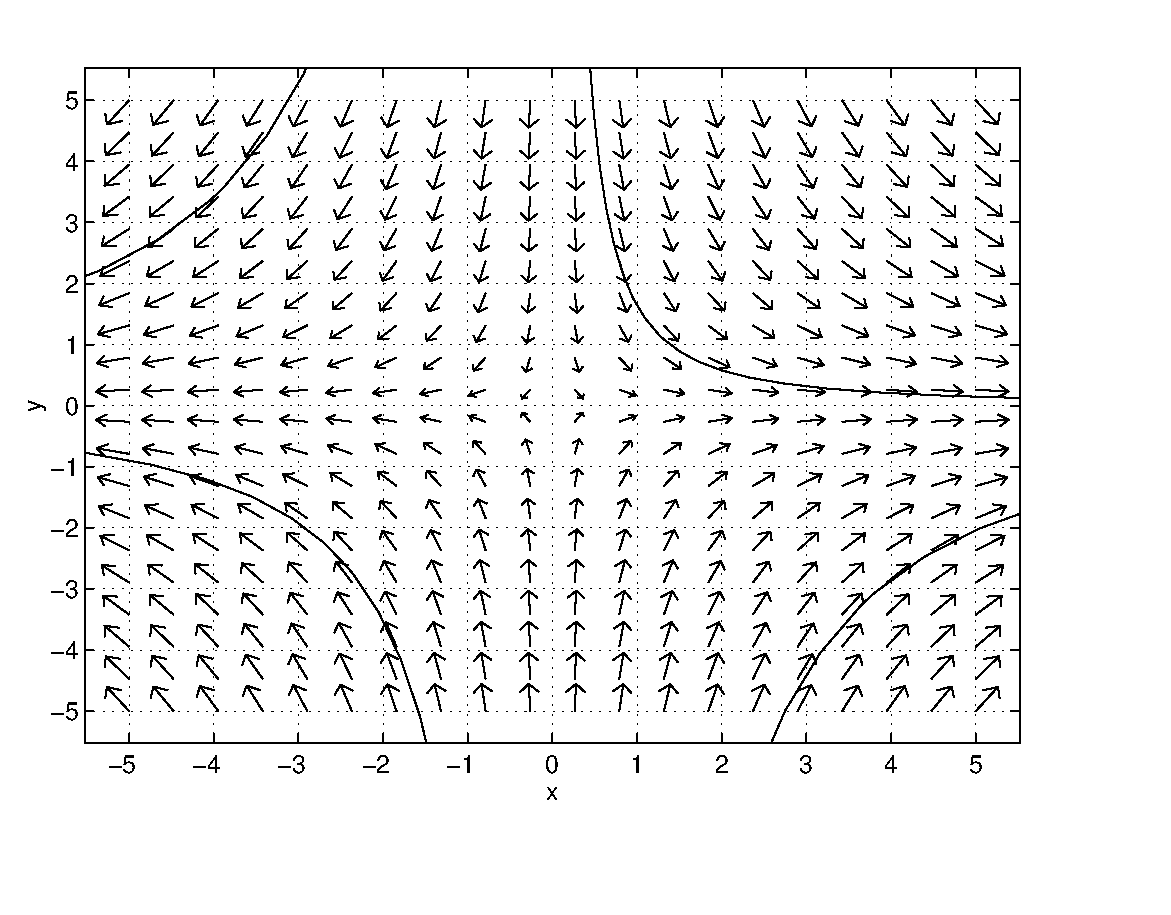
\psfig{file=exfigure/6-3-3a.eps,width=1.8in}
                       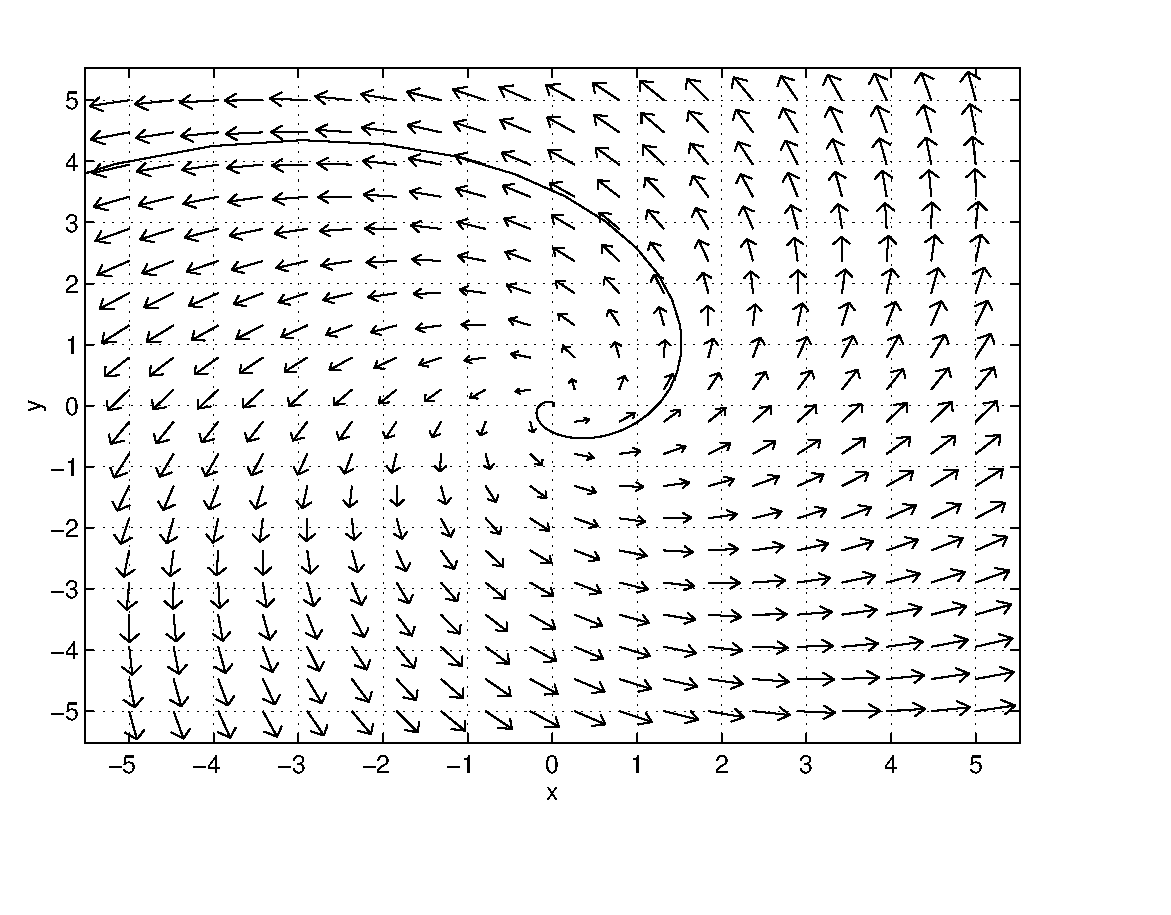
\psfig{file=exfigure/6-3-3b.eps,width=1.8in}
                       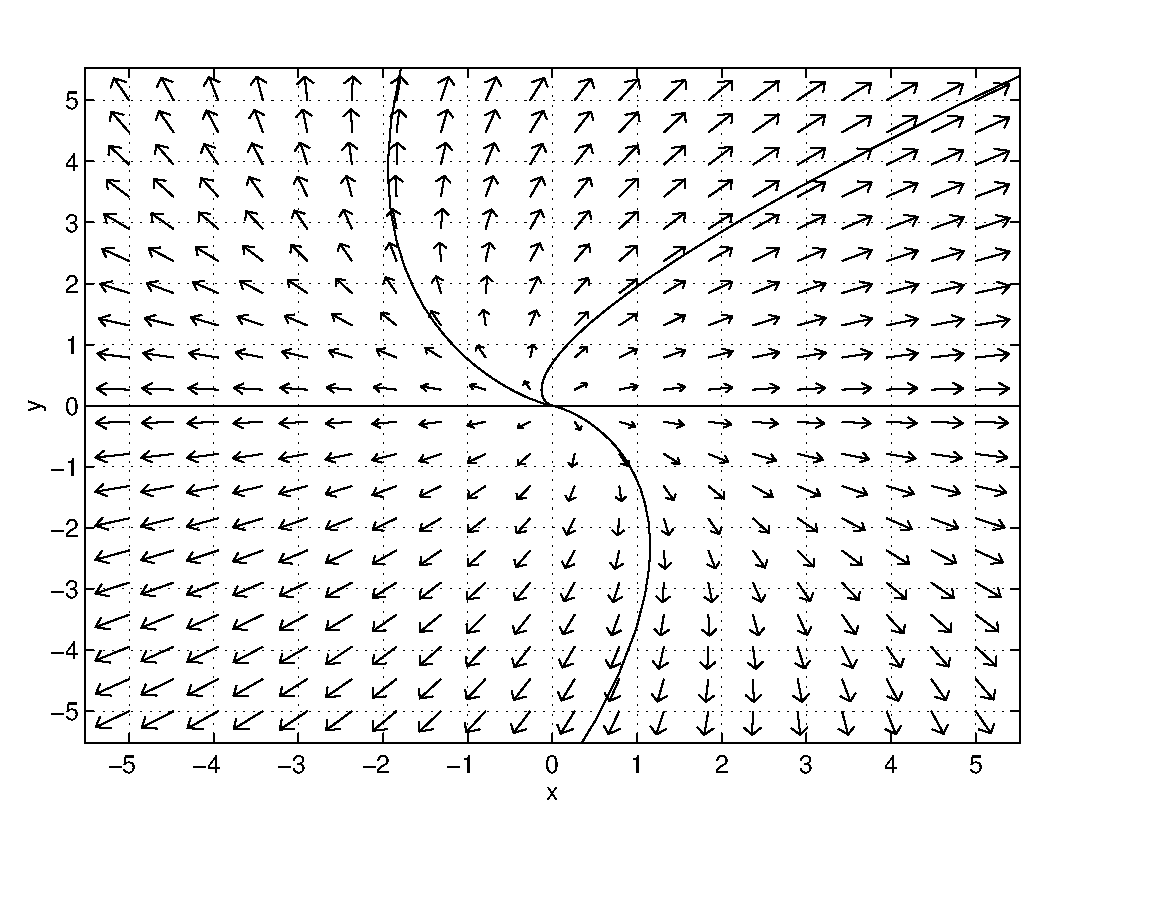
\psfig{file=exfigure/6-3-3c.eps,width=1.8in}}
                \exercapthree{c6.3.3}
\end{figure}



\end{solution}
\end{exercise}

\AEXER

\begin{exercise} \label{c6.4.a1}
Let $A$ be an $n\times n$ matrix.  Prove that $e^A$ is invertible.
\end{exercise}

\end{document}
